\section{Results and Evaluation}

\begin{frame}{Model Selection \& Metrics}
    \textbf{Validation Baseline Comparison:}
    \begin{itemize}
        \item \textbf{Random Forest:} Accuracy 0.6843 | ROC AUC 0.7023
        \item \textbf{XGBoost:} Accuracy 0.6817 | ROC AUC 0.7033
        \item \textbf{Champion Model: Random Forest} (Chosen for interpretability).
    \end{itemize}
    \vspace{0.3cm}
    \textbf{Final Test Performance ($N=3855$):}
    \begin{itemize}
        \item \textbf{Accuracy:} 67.32\%  | \textbf{ROC AUC:} 0.6998
        \item Metrics align with validation results, confirming \textbf{no overfitting}.
    \end{itemize}
\end{frame}

\begin{frame}{Final Test: Confusion Matrix}
    \begin{columns}
        \begin{column}{0.4\textwidth}
            \textbf{Recall Asymmetry:}
            \begin{itemize}
                \item \textbf{Missed (0):} High Recall (85\%). Model confident in misses.
                \item \textbf{Made (1):} Conservative behavior. High Precision (71\%) but low Recall (46\%).
            \end{itemize}
        \end{column}
        \begin{column}{0.6\textwidth}
            \begin{figure}
                \centering
                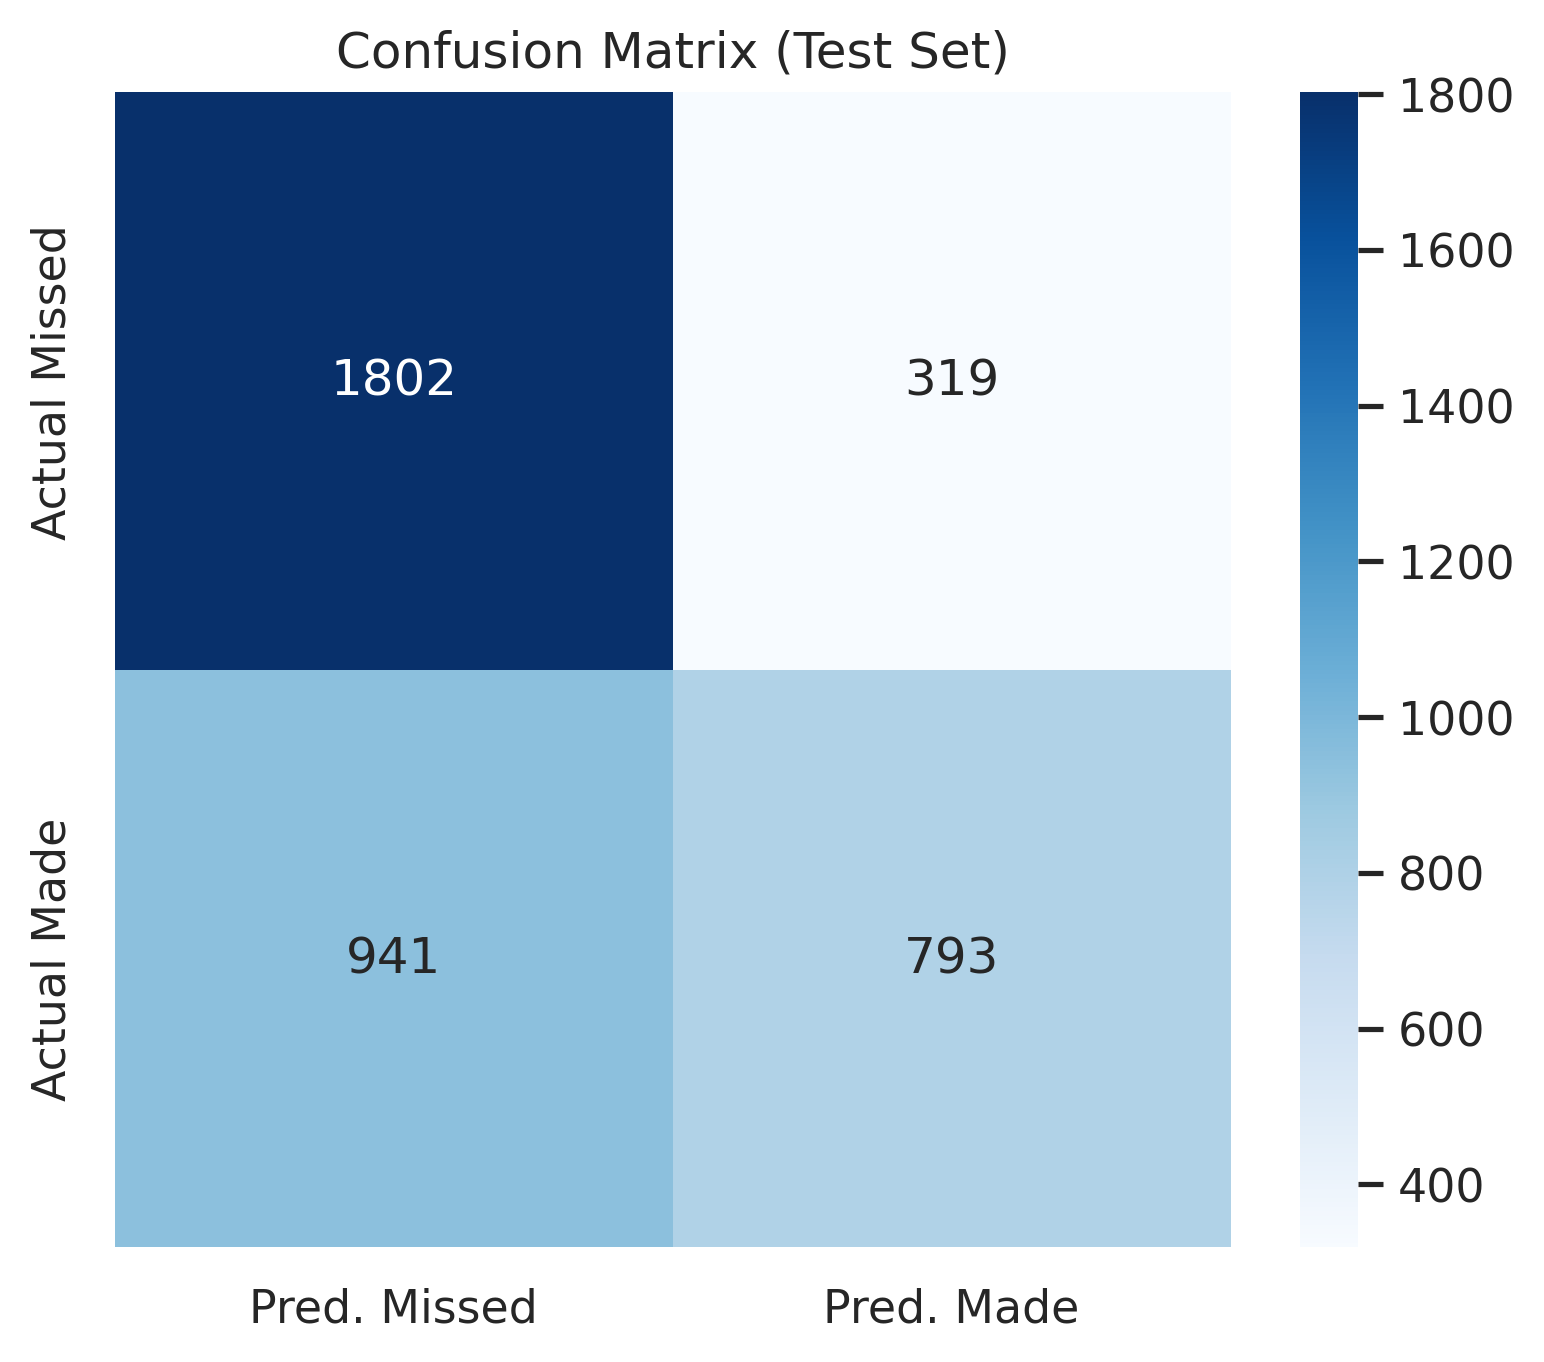
\includegraphics[width=0.9\textwidth]{img/confusion_matrix.png}
            \end{figure}
        \end{column}
    \end{columns}
\end{frame}

\begin{frame}{Qualitative Error Diagnostics}
    \textbf{Spatial Analysis of Errors:}
    \begin{itemize}
        \item Avg distance (Incorrect): 14.18 ft. | Avg distance (Correct): 13.19 ft.
    \end{itemize}
    \vspace{0.3cm}
    \textbf{The Mid-Range Problem:}
    \begin{itemize}
        \item Algorithm struggles as distance increases into the \textbf{mid-range}.
        \item \textbf{Why?} Tactical uncertainty heavily influenced by defender pressure.
        \item Contextual defensive data is absent from dataset, creating a natural ceiling for predictive reliability.
    \end{itemize}
\end{frame}